\section{Conic Sections in Polar Coordinates}
  \begin{theorem}
    Let $F$ be a fixed point (called the \textbf{focus}) and $l$ be a fixed line  (called the \textbf{directrix}). Let $e$ be a fixed positive number (called the \textbf{eccentricity}). The set of all points P in the plane such that
    $$\frac{|PF|}{|Pl|}=e \ \ \ \text{\footnotesize(the ratio of the distance from $F$ to the distance from $l$ is the constant e})$$
    is a conic section. The conic is
    \begin{enumerate}
      \item an ellipse if $e<1$
      \item a parabola if $e=1$
      \item a hyperbola if $e>1$
    \end{enumerate}
  \end{theorem}
  \begin{center}
      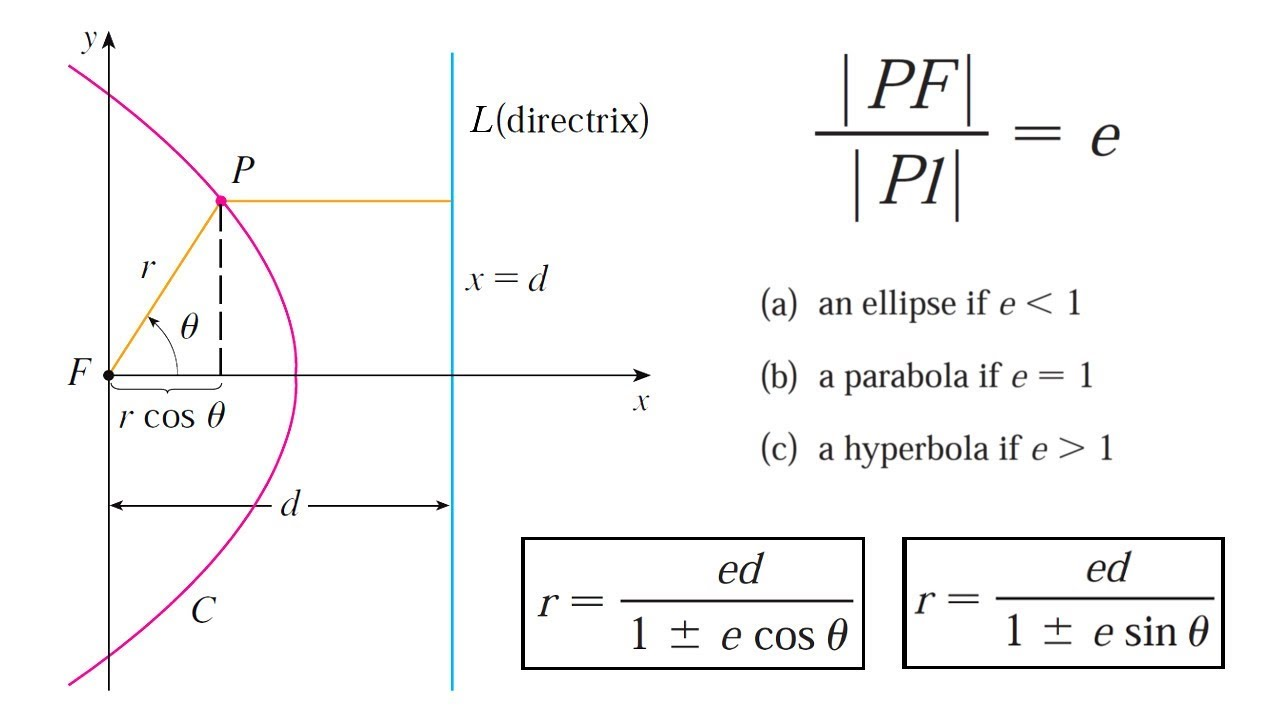
\includegraphics[width=250pt]{eccentricity.jpg}
    \end{center}
  \begin{theorem}
    A polar equation of the form
    $$r=\frac{ed}{1\pm e\cos\theta}\ \ \ \text{or}\ \ \ r=\frac{ed}{1\pm e\sin\theta}$$
    represents a conic section with eccentricity $e$ and distance $d$ from the center to the directrix, with the focus at the origin. The conic is an ellipse if $e<1$, a parabola if $e=1$, or a hyperbola is $e>1$.
  \end{theorem}
  \begin{center}
      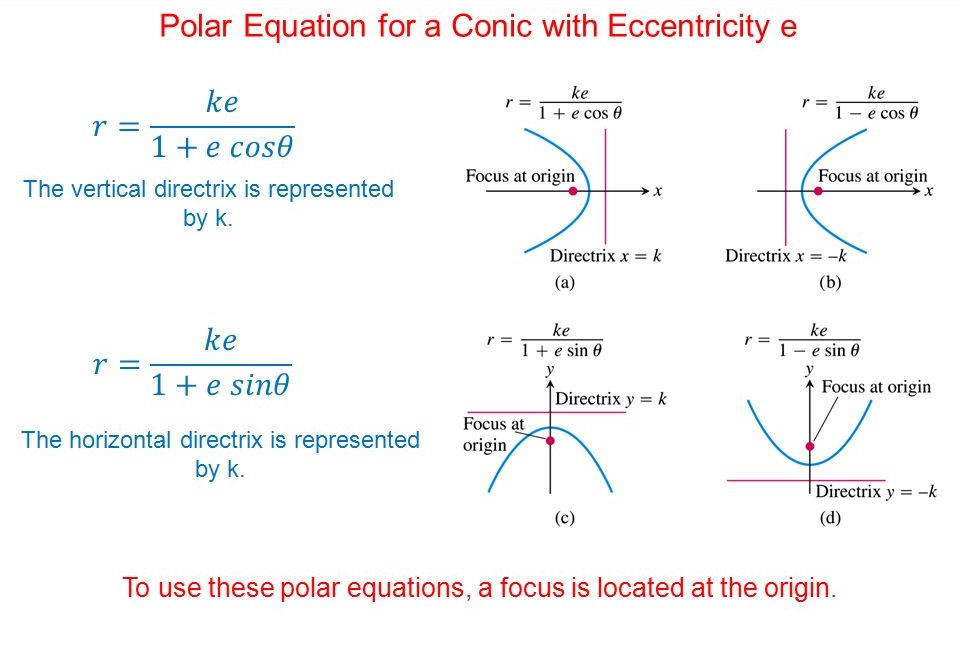
\includegraphics[width=300pt]{polar_conic.jpg}
  \end{center}
   Use ``$\cos\theta$'' when the conic section opens rightward or leftward, and use ``$\sin\theta$'' when the conic section opens upward or downward. Use ``$+$'' if the conic section opens leftward or downward, and use ``$-$'' if the conic section opens righttward or upward.
  \begin{example}
    Find a polar equation for a parabola that has its focus at the origin and whose directrix is the line $y=-6$.
  \end{example}
  \begin{solution}
    The eccentricity $e=1$ because the conic section is a parabola, and the distance from the center to the directrix is $d=6$. The directrix is on the $y$-axis and is underneath the center, so the parabola opens upward. Therefore, we use the ``$\sin\theta$'' equation and use ``$-$'' in the denominator. The polar equation of the parabola is $$r=\frac{6}{1-\sin\theta}$$.
  \end{solution}
  \begin{example}
    A conic is given by the polar equation
    $$r=\frac{10}{3-2\cos\theta}$$
    Find the eccentricity, identify the conic, and locate the directrix.
  \end{example}
  \begin{solution}
    Divide the numerator and denominator by 3 to get
    $$r=\frac{\frac{10}{3}}{1-\frac{2}{3}\cos\theta}$$
    This represents an ellipses with eccentricity $e=\frac{2}{3}$. Since $ed=\frac{10}{3},$
    $$d=\frac{\frac{10}{3}}{e}=\frac{\frac{10}{3}}{\frac{2}{3}}=5$$
    so the directrix has Cartesian equation $x=-5$. When $\theta=0,\ r=10$; when $\theta=\pi,\ r=2$, so the vertices have polar coordinates $(10,0)$, and $(2,\pi)$.
  \end{solution}
